\subsection{Experimentación Final}

Para concluir este trabajo, tomamos el algoritmo de backtracking, el algoritmo goloso, el de busqueda local 1 y GRASP 1 y mediremos las diferencias de performance y de tiempos en cada uno para intentar sacar conclusiones.

Comenzaremos con un pequeño experimento variando $n$. Tomaremos grafos completos con $k = 5$, pesos aleaotrios en las aristas y variando la cantidad de nodos desde $1$ a $19$ y mediremos cuales son los k-PMP encontrados por cada algoritmo.

Los resultados arrojados por la experimentación pueden verse en el siguiente grafico:

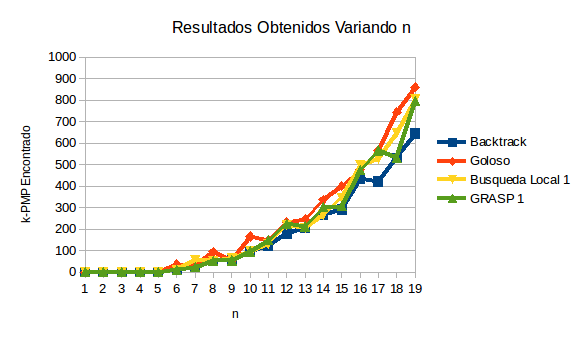
\includegraphics[scale=0.5]{Con/performance1.png}

Lo primero que podemos observar es que para casos triviales con $n <= k$ todos son capaces de encontrar la respuesta optima.

Lo segundo que podemos observar, es que salvo un caso, el algoritmo goloso siempre pareciera ser el que encuentra las peores soluciones, llegando a obtener una respuesta un $33 \%$ alejada de la optima en el caso de $19$ nodos. (k-PMP encontrado por el backtrack: 644, k-PMP encontrado por la heuristica golosa: 860).

Las respuestas obtenidas por la busqueda local y el GRASP, resultan en general, en mucho mejores k-PMPs, desviandose hasta un $10\%$ de la respuesta por backtracking.

Ademas de estos 19 casos, podemos ver que el algoritmo goloso encuentra $6$ soluciones exactas (las 5 triviales y una para $n = 9$), la busqueda local encuentra $10$ respuestas exactas y el GRASP encuentra $11$ respuestas exactas. Si bien este el set de datos no es muy significativo, ya es posible ver las ventajas que representan las dos ultimas heuristicas frente a la primera.

Ademas, para estos 19 casos, medimos los tiempos que tardan en obtener una respuesta:

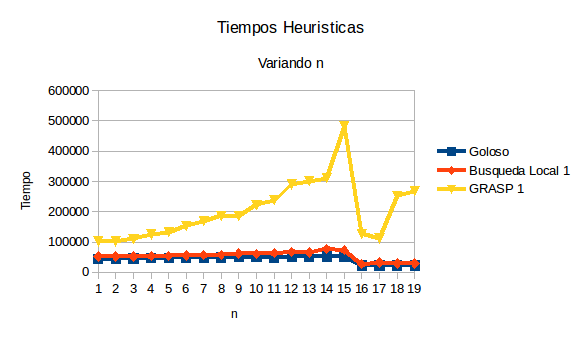
\includegraphics[scale=0.5]{Con/tiempos1Back.png}

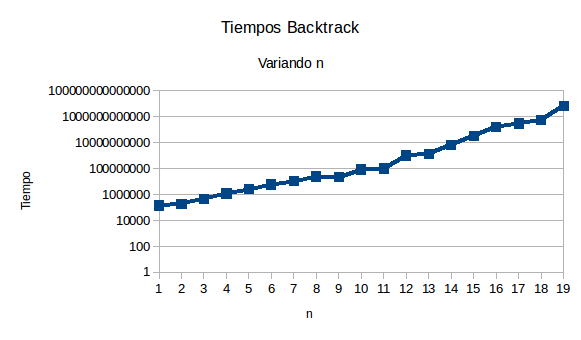
\includegraphics[scale=0.5]{Con/tiempos1Otros.png}

Como era de esperar, mietras que las heuristicas escalan de manera mas o menos polinomial, el backtracking escala de manera exponencial ascendiendo un orden de magnitud cada vez que asciende en uno el valor de $n$, hasta el punto que pasados los $19$ nodos, los tiempos empiezan a ser inviables.

\subsection{Experimentación sobre grafos faciles}

En esta sección buscaremos determinar cuanto mejor es el GRASP sobre la familia de grafos para la que fue entrenada (grafos completos, con aristas tomadas al azar entre $1$ y $100$), para intentar mostrar las ventajas que representa frente a los otros algoritmos. Para eso correremos el Backtrack sobre $100$ grafos de $19$ nodos completos, con pesos en las aristas aleaotrios entre 1 y 100 y $k = 4$ y veremos en cuantos casos cada algoritmo encuentra la respuesta exacta, e intentaremos sacar concluciones sobre los datos obtenidos.

Las respuestas obtenidas son las siguientes:

\includegraphics[scale=0.5]{Con/faciles.png}

\subsection{Experimentación sobre grafos dificiles}

Para poner realmente a prueba los tres algoritmos diseñamos una nueva familia de grafos que consideramos difil de resolver para nuestros algoritmos. Los grafos de esta famila se describien asi: dada una cantidad de nodos $n$ y una cantidad de aristas igual a $n*(n-1)/2$, tomamos la mitad de las aristas con peso igual a $1$ y la otra mitad con peso igual a $100000$. Ademas k debe ser igual a $n/6$.

Fijamos $n=250$ y tomamos $100$ de estos grafos. Para ejemplificar lo obtenido, se incluyen las respuestas obtenidas en tres instancias del problema.

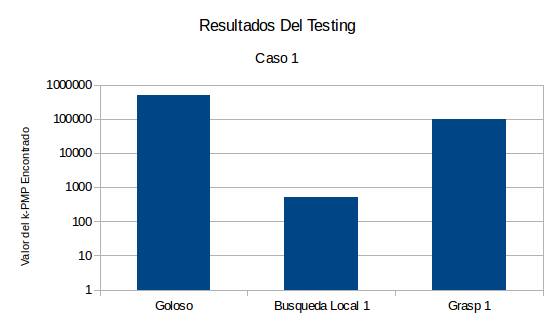
\includegraphics[scale=0.5]{Con/dificil1.png}

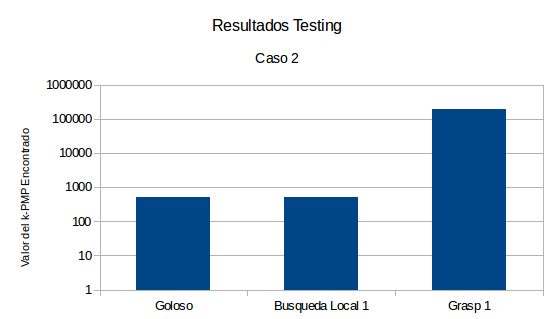
\includegraphics[scale=0.5]{Con/dificil2.png}

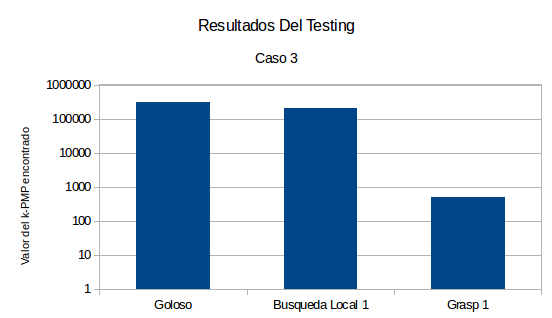
\includegraphics[scale=0.5]{Con/dificil3.png}

Notar que los graficos estan en escala logaritmica, lo que quiere decir, que en el caso uno por ejemplo, el algoritmo goloso (k-PMP encontrado: 500502) y el GRASP (k-PMP encontrado: 100501) obtuvieron respuestas aproximadamente un $100100 \%$ peor que la Busqueda local (k-PMP encontrado: 501).

De ahora en adelante, en este apartado, llamaremos a una respuesta, "buena", si se encuentra entre 0 y $1000$.

Analizando los datos, vemos que el algoritmo goloso solo logró llegar a una respuesta buena, 4 veces, mientras que el tanto el grasp, como la busqueda local lograron obtener $51$ respuestas buenas en estos grafos (no necesariamente en el mismo grafo, como puede notarse en las figuras)

Si bien un $50 \%$ de respuestas buenas puede ser una cantidad aceptable, una posible solución para mejorarla, sería entrenar nuevamente al GRASP con este set de datos, y intentar conseguir un nuevo $\alpha$ y un nuevo $z$ de tal manera que se maximicen las posivilidades de encontrar la respuesta. Otro posible solición sería encontrar alguna propiedad especifica para esta familia de grafos que facilite su resolución con alguna otra heuristica mas apropiada.

\section{Conclusión}

Concluimos que dado que el problema de $k-PMP$ resulta extremadamente dificil de resolver de manera exacta, es posible encontrar heuristicas que nos aproximen a una buena solución en un tiempo razonable, siempre teniendo en cuenta que pagamos tiempo con exactitud.

Vimos que la técnica de Metaheurística GRASP es una combinación válida entre distintos esquemas de algoritmos y trata de combinarlas para explorar el espacio de soluciones de una manera eficiente. En nuestro caso particular vimos que la implementación de GRASP 1, lograba ser bastante efectivo dentro de la familia de grafos para las fue entrenado. Aunque como se vio en el apartado de "Experimentación sobre un grafo dificil" al ser utilizado para resover casos patologicos, puede obtener respuestas equiparables con un algoritmo mas simple de busqueda local.

Como trabajo futuro, podría intentar implementarse un backtracking que primero corra una buena metaeuristica de manera de comenzar con una buena solución inicial. De esa manera, las podas que podría aplicar el algoritmo, serían en teoría mucho mejores, lo que sin duda ayudaría a bajar los tiempos de ejecución.